\section{Auswertung}
\label{sec:auswertung}

\begin{figure}
    \centering
    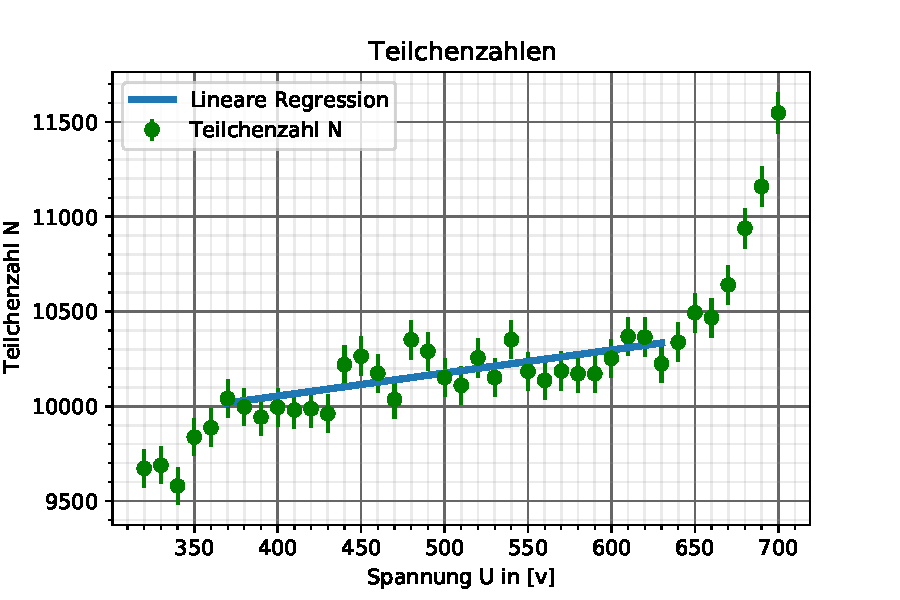
\includegraphics{kennlinie.pdf}
    \caption{Teilchenzahlen im Geiger-Müller-Zählrohr}
    \label{fig:teilchenzahl}
  \end{figure}
Um die Plateau-Steigung zu ermittlen wurde mittels linearer Regression ein polynom ersten Grades der 
Form $f(x)=ax+b$ durch die Messpunkte gelegt:
\begin{center}
    $f(x)=(1.215\pm0.256)x + (9567.924\pm125.414)$ $\rightarrow$ $D_f=\{x\in\mathbb{R} \vert 360\le x\le620\}$    
\end{center}
